\documentclass{article}

\usepackage{amsmath}
\usepackage{float}
\usepackage{csvsimple}

\usepackage{graphicx}
\graphicspath{ {../results/} }

\usepackage[style=numeric, backend=bibtex8]{biblatex}
\addbibresource{citations.bib}

\begin{document}

  \title{Linear Time Generation of Simulated Wireless Sensor Networks with Random Geometric Graphs}
  \author{Luke Wood}
  \maketitle

  \section{Executive Summary}
	Wireless Sensor Networks (WSNs) are a group of ad hoc wireless devices that communicate amongst themselves.
	They are incredibly expensive to develop and test which makes them a great candidate for simulation as a preliminary way to gather data.
	Vlady Ravelomananana and Hichem Kenniche from the University of Paris first explored the concept of using random geometric graphs (RGGs) to attempt to model wireless sensor networks \cite{kenniche2010random}.
  At the moment random geographic graphs are the state of the art method for simulating WSNs.
	In this project I will use RGGs as a way to gather valuable information about how wireless sensor networks will possibly function and communicate.

  \subsection{Introduction and Summary}
	Through a series of three reports	I will be analyzing RGGs in the following ways as an attempt to gain some insight into the behavior of wireless sensor networks:
	\begin{enumerate}
		\item Generating RGGs on the geometries of a unit square, unit disc, and unit sphere
		\item Color the generated graph in linear time using smallest vertex last ordering
		\item Find the terminal clique in the generated RGGs
		\item Find a selection of bipartite subgraphs producted by an algorithm for coloring
	\end{enumerate}
	This report is the first of the series and will describe an implementation for a linear time algorithm to generate graphs consisting of N vertices with an average degree of A on the geometric topologies of: unit square, unit disc, unit sphere.
	Some tables are included to display some metrics for generated  RGGs of various size to display the performance of the generation algorithm.
	The square topology generation algorithm runs in approximately 15 seconds for graph size 100000 which is fast given the large input size.

	\begin{center}
	  \begin{table}[H]
      \csvautotabular{../results/square/benchmarks/data.csv}
			\caption{Data on Graphs Generated with the Square Topology}
		\end{table}
	\end{center}

	The disc topology also runs in linear time but the constant factor is much larger than that of the square topology.
	This is due to some overhead that I incurred when generating the points themselves.
	Despite the algorithm being slower than the square version, it still terminated in 48 seconds for 100000 nodes.
	This is an acceptable runtime.

  \begin{center}
	  \begin{table}[H]
      \csvautotabular{../results/disc/benchmarks/data.csv}
			\caption{Data on Graphs Generated with the Disc Topology}
		\end{table}
	\end{center}

  The sphere generation ran in .....

  \begin{center}
	  \begin{table}[H]
      \csvautotabular{../results/sphere/benchmarks/data.csv}
			\caption{Data on Graphs Generated with the Sphere Topology}
		\end{table}
	\end{center}

	One interesting thing to notice in the above tables is that as the number of nodes grows the real average degree converges on the expected average degree.
	The lower the number of nodes the further from the expected average degree the real number is.
	This happens due to there not being enough nodes in the graph for the real radius to reach the expected value.

	Going forwards I will continue to implement linear time algorithms to solve the problems at hand.
	I will possible move from python to the Elixir programmign language to utilize the high level of parralelism that comes from immutable data.

  Currently, my implementation has support for:
  \begin{enumerate}
		\item Generating a RGG with a unit square topology
		\item Generating a RGG with a unit disc topology
    \item Generating a RGG with a unit sphere topology
		\item Converting RGGs to an Adjacency List
		\item Serializing Adjacency Lists to files
  \end{enumerate}
  Being able to serialize the Adjacency Lists to files is a noteworthy feature as if there are algorithms that require faster runtimes than a dynamically typed language can support (such as python) we can still generate the RGGs from the generation implementation  and use them in other computation ecosystems.

  \subsection{Programming Environment Description}
		The implementation of the algorithm used to gather the data supporting this report was gathered on a 15 inch Macbook pro 2017 with a 2.9 GHz Intel Core i7 processor and 16 GB of RAM.
		The computer is running macOS High Sierra.
		The graph generation is written in python 3 as generating and connection a graph is not super computationally expensive with even decently large inputs such as 100000.
		The later algorithms may be implemented in a different language such as Elixir to get high levels of concurrency and higher efficiency due to type inference (as opposed to pythons dynamic typing).
  \section{Reduction to Practice}
		In this section I will discuss how the transition from theory to implementation went.
		I will discuss optimizations I made as well as optimizations that I was aware that I could make but decided not to for reasons.
	\subsection{Data Structure Design}
		In the generation portion of this project I use several different data structures.
		The first one is a python object of custom type node.
		This basically serves as a tuple of values consisting of an X location, a Y location, a list of nodes, and a node number.
		All of these are used during the connecting of the nodes in graph generation excluding node number.
		Node number is assigned during object construction time and is only used when converting the list of nodes into an adjacency list.
		This data structure could be used interchangeably with a statically indexed tuple instead of an object to avoid any overhead associated with objects in python, however I believe that the readability gained from using a custom node class heavily outweighs the marginal performance benefit gained from using a statically indexed tuple.
		Both of these data structures provide $O(1)$ read and write operations.
		If we were to generate gigantic graphs then an argument could be made to switch over the statically indexed tuples to reduce the access time for attributes by a bit.

		The second mentioned data structure is the adjacency list.
		Adjacency lists are an efficient graph representation that we will use in the subsequent reports.
		Adjacency lists require only $O(v*e)$ storage as opposed to the $O(v^2)$ required for adjacency matrixes.
		This is handy in situations where the expected average number of edges is significantly lower than the number of nodes in the graph.
		Despite the huge potential savings on storage, the only sacrifice adjacency lists make is in the lookup operation to determine if there is an edge between two nodes.
		This takes $O(e)$ in an adjacency list as opposed to $O(1)$ in an adjacency matrix.

	\subsection{Algorithm Description}
		In the following sections I will give a detailed analysis of the algorithms used in this project.
		I will discuss the runtimes of each algorithm in terms of $\Omega$, $O$, and $\Theta$ when relevant.

    	\begin{center}
    		\begin{table}
    			\begin{tabular}{ |c|c| }
    				\hline
    				Algorithm & $O$ \\
    				\hline
    				Square Point Generation & $O(n)$ \\
    				\hline
    				Disc Point Generation & $O(n)$ \\
    				\hline
            Sphere Point Generation & $O(n)$ \\
            \hline
    				Node Connection & $O(n)$ \\
    				\hline
    			\end{tabular}
          \caption{big O of all of the algorithms described}
    		\end{table}
    	\end{center}

  \subsection{Square Point Generation}
		The algorithm to generate the points in the unit square topology is incredibly simple.
		Simply pick two random numbers between 0 and 1 for all nodes.

  \subsection{Disc Point Generation}
		Generating the points on the Disc topology is slightly more challenging than generating the points for the square topology.
    The algorithm for generating points in the unit disc is as follows:
    Pick a random x and y between 0 and 1.
    Calculate the distance between that point and the center of the unit circle (0.5, 0.5).
    If the distance is less than or equal to .5 we take this point, otherwise we generate another point.

	\subsection{Node Connection}
		In order to ensure that average degree of the nodes is close to the desired average degree we define a radius surrounding each node.
		The formulas to find the radius for each topology is derived from the equations found in the paper Bipartite Grid Partitioning of a Random Geometric Graph\cite{chen2017bipartite}.
		The formula used to find this radius varies for each graph tolopogy and can be found in the table displayed below:

		\begin{tabular}{ |c|c|c| }
				\hline
				Topology & Equation Used to Derive Radius & Radius Equation \\
				\hline
				Unit Square & $d(G) \approx N\pi r^2 $ & $r = sqrt(\dfrac{d(G)}{N\pi})$ \\
				\hline
				Unit Disc & $r = sqrt(\dfrac{d(G)}{N\pi})$ & $r = sqrt(\dfrac{d(G)}{N})/2$ \\
				\hline
				Unit Sphere & $r = sqrt(\dfrac{d(G)}{N})/2$ & $r = sqrt(\dfrac{d(G)}{N})/4$ \\
				\hline
		\end{tabular}
    I did not personally derive the unit sphere radius formula.
    I instead looked at the implementation of Ian Johnson\cite{ianjjohnson}.
	\subsection{Conversion From Node List to Adjacency Matrix}
		The algorithm to convert from a list of the node class I defined to an adjacency list is extremely straight forward.
		The algorithm consists of a pair of nested map operations.
		The first operation maps each node to it's edges list.
		The second operation maps each item of the edge lists to it's respective node number.
		This quickly yields an $O(v*e)$ algorithm to change my node list to an adjacenecy matrix.
		If the performance of $O(v*e)$ is deemed unacceptable in the future, then we can simply append the node number to the list of edges as opposed to a pointer to the node object deeming the second map operation unneccesary yieling an $O(v)$ algorithm.


  \subsection{Algorithm Engineering}
	  Originally I had a brute force algorithm that ran in $O(n^2)$ time.
	  This quickly became problematic as the algorithm took upwards of 200 seconds to run on input size of only 12,000.
	  \begin{figure}[H]
		\centering
		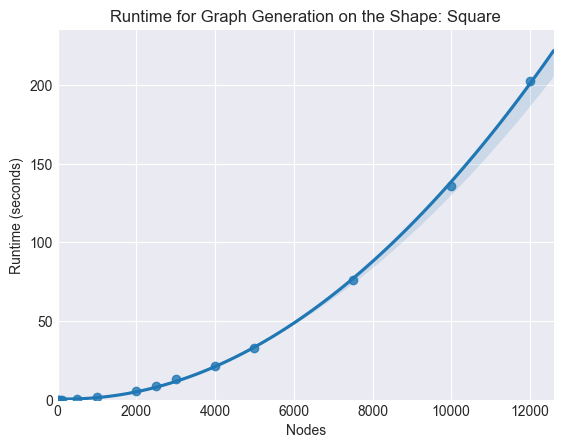
\includegraphics[width=1 \textwidth]{square/runtime/runtime_chart_naive}
		\caption{Runtimes of the $O(n^2)$ Algorithm}
	  \end{figure}


	  To fix this, I overhauled the algorithm to be $O(n)$.
	  I did this by implementing the cell method described above in the Algorithm Description section as well as in Chen's paper Bipartite Grid Partitioning of a Random Geometric Graph\cite{chen2017bipartite}.
	  \begin{figure}[H]
  		\centering
  		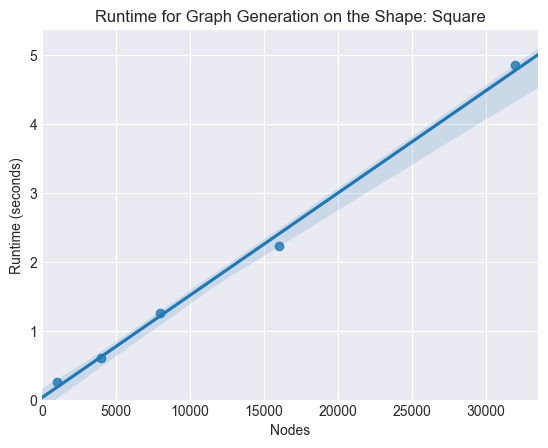
\includegraphics[width=1 \textwidth]{square/runtime/runtime_chart}
  		\caption{Runtimes of the $O(n)$ Algorithm}
	  \end{figure}

	  I have also included a table to compare some of the runtimes for the same size inputs below.

	  \begin{center}
	  \begin{table}[H]
		\begin{tabular}{ |c|c|c| }
			\hline
			Nodes & $O(n^2)$ & $O(n)$ \\
			\hline
			  1000 & 0.258400 & 0.657174 \\
			  \hline
			  2000 & 0.382116 & 2.630040 \\
			  \hline
			  3000 & 0.473916 & 5.874501 \\
			  \hline
			  5000 & 0.831753 & 16.809004 \\
			  \hline
			  10000 & 1.560216 & 65.398991 \\
			\hline
		\end{tabular}
		\caption{Runtimes of the $O(n)$ and $O(n^2)$ algorithms in seconds}
	  \end{table}
	  \end{center}

	  The $O(n)$ algorithm is far superior even on small input sizes such as 1000.

    I originally was using a python object to store the data of each node but instead switched over to a statically indexed tuple.

	\subsection{Verification}
		One way that we verified our results was checking the distribution of edge densities in our graph.
		We expect to see a gaussian distribution in the edge densities with the center being around our calculated radius.
		We can also verify the runtime of our algorithms by plotting the input size on the x axis and the runtime on the y axis.
		If we have a linear algorithm we should be able to fit the distribution of points to a linear equation with minimal error.
		Both of these verification methods were successful and can be seen in the results section of this report.

  \subsubsection{Visualizing the Points}
    A simple way to validate that the points are distributing correctly is by plotting out the points in a scatter plot.
    Early on I had a bug where I was accidentally distributing the points around the radius of the unit disc instead of evenly inside the unit disc.
    I found this by scatter plotting the points and seeing that they were clearly around the circumference of the circle.
    The following two figures

    \begin{figure}[H]
      \centering
      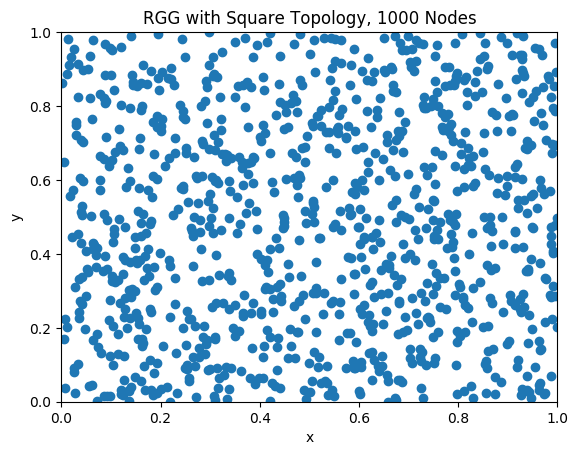
\includegraphics[width=1 \textwidth]{square/drawing/nodes.png}
      \caption{1000 Points on the Square Topology}
    \end{figure}
    The points are uniform randomly distributed over the square topology as we can see in the above figure.
    \begin{figure}[H]
      \centering
      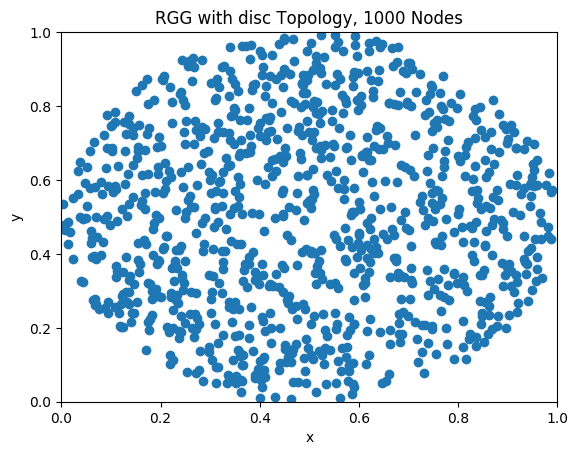
\includegraphics[width=1 \textwidth]{disc/drawing/nodes.png}
      \caption{1000 Points on the Disc Topology}
    \end{figure}
    The points are uniform randomly distributed over the unit circle in the disc topology.
    \begin{figure}[H]
      \centering
      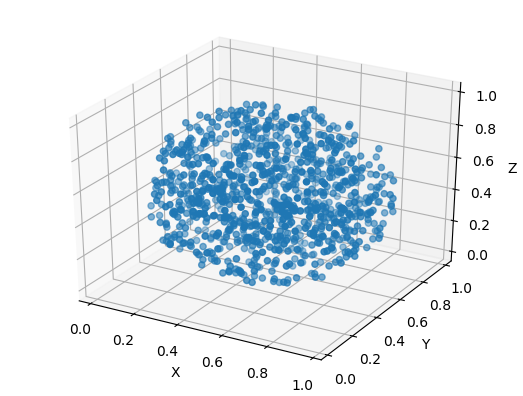
\includegraphics[width=1 \textwidth]{sphere/drawing/sphere_drawing.png}
      \caption{1000 Points on the Sphere Topology}
    \end{figure}
    The same is true for that of the unit sphere.

\section{Result Summary}
  \subsection{Edge Density}
  As expected I got a gaussian distribution for my edge densities.
  This is apparent in the attached edge distribution charts for each topology
  \begin{figure}[H]
    \centering
    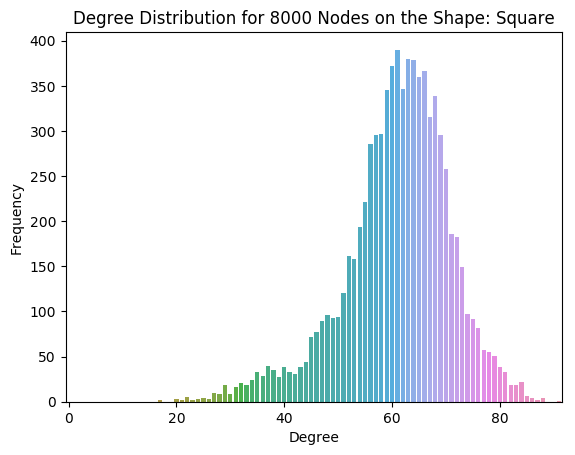
\includegraphics[width=1 \textwidth]{square/edge_density/8000_64.png}
    \caption{Edge Densities of an 8000 Node Graph with E(Degree)=64 on Topology Square}
  \end{figure}

  \begin{figure}[H]
    \centering
    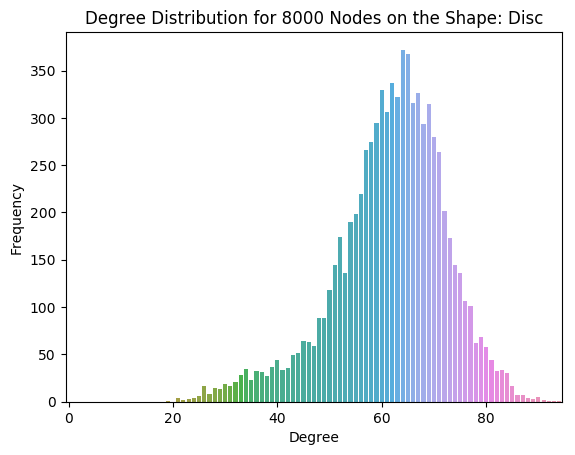
\includegraphics[width=1 \textwidth]{disc/edge_density/8000_64.png}
    \caption{Edge Densities of an 8000 Node Graph with E(Degree)=64 on Topology Disc}
  \end{figure}
  All of the edge density dsitributions follow a gaussian distribution which is what we expected.
  This seems like a good outcome for this portion of the results.
  \subsection{Performance Rates}
  All of my algorithms ran in $O(n)$ time.
  There was variance between the runtime of the different topologies due to the way the points were generated.
  \begin{center}
	  \begin{table}[H]
		  \csvautotabular{../results/shared/generation_speeds.csv}
		  \caption{Comparison of Runtimes of Generating the Different Topologies}
	  \end{table}
  \end{center}

  \begin{figure}[H]
    \centering
    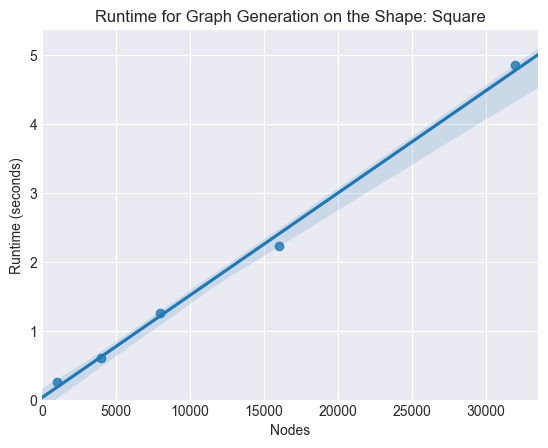
\includegraphics[width=1 \textwidth]{square/runtime/runtime_chart}
    \caption{Runtimes of the $O(n)$ Algorithm}
  \end{figure}

  \begin{figure}[H]
    \centering
    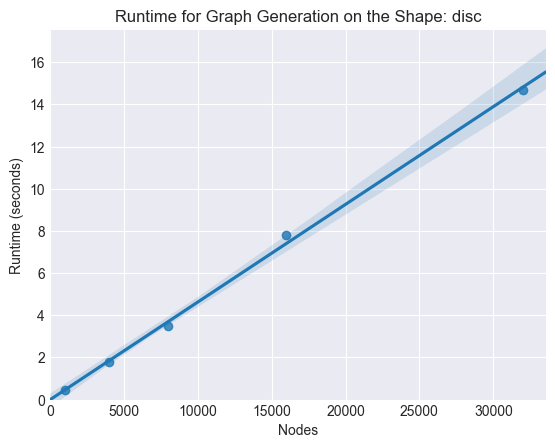
\includegraphics[width=1 \textwidth]{disc/runtime/runtime_chart}
    \caption{Runtimes of the $O(n)$ Algorithm}
  \end{figure}

\printbibliography

\end{document}
